\documentclass[12pt]{article}
\usepackage[utf8]{inputenc}
\usepackage{graphicx} % Allows you to insert figures
\usepackage{amsmath} % Allows you to do equations
\usepackage{fancyhdr} % Formats the header
\usepackage{geometry} % Formats the paper size, orientation, and margins
\usepackage[T1]{fontenc}
\usepackage[polish]{babel}
\usepackage[utf8]{inputenc}
\usepackage{float}
\linespread{1.25} % about 1.5 spacing in Word
\setlength{\parindent}{0pt} % no paragraph indents
\setlength{\parskip}{1em} % paragraphs separated by one line
\usepackage[style=authoryear-ibid,backend=biber,maxbibnames=99,maxcitenames=2,uniquelist=false,isbn=false,url=true,eprint=false,doi=true,giveninits=true,uniquename=init]{biblatex} % Allows you to do citations - does Harvard style and compatible with Zotero
\urlstyle{same} % makes a nicer URL and DOI font 
\AtEveryBibitem{
    \clearfield{urlyear}
    \clearfield{urlmonth}
} % removes access date
\AtEveryBibitem{\clearfield{month}} % removes months in bibliography
\AtEveryCitekey{\clearfield{month}} % removes months in citations
\renewbibmacro{in:}{} % Removes the "In" before journal names

\renewbibmacro*{editorstrg}{%from biblatex.def
  \printtext[editortype]{%
    \iffieldundef{editortype}
      {\ifboolexpr{
         test {\ifnumgreater{\value{editor}}{1}}
         or
         test {\ifandothers{editor}}
       }
         {\bibcpstring{editors}}
         {\bibcpstring{editor}}}
      {\ifbibxstring{\thefield{editortype}}
         {\ifboolexpr{
            test {\ifnumgreater{\value{editor}}{1}}
            or
            test {\ifandothers{editor}}
          }
            {\bibcpstring{\thefield{editortype}s}}%changed
            {\bibcpstring{\thefield{editortype}}}}%changed
         {\thefield{editortype}}}}}

\renewbibmacro*{byeditor+others}{%from biblatex.def
  \ifnameundef{editor}
    {}
    {\printnames[byeditor]{editor}%
     \addspace%added
     \mkbibparens{\usebibmacro{editorstrg}}%added
     \clearname{editor}%
     \newunit}%
  \usebibmacro{byeditorx}%
  \usebibmacro{bytranslator+others}}
  % The commands above from lines 20-49 change the way editors are displayed in books
\AtEveryBibitem{%
  \clearlist{language}%
} % removes language from bibliography
\citetrackerfalse 
% Removes ibids (ibidems)
\DeclareNameAlias{sortname}{family-given} % Ensures the names of the authors after the first author are in the correct order in the bibliography
\renewcommand*{\revsdnamepunct}{} % Corrects punctuation for authors with just a first initial
\addbibresource{Example.bib} % Tells LaTeX where the citations are coming from. This is imported from Zotero
\usepackage[format=plain,
            font=it]{caption} % Italicizes figure captions
\usepackage[english]{babel}
\usepackage{csquotes}
\renewcommand*{\nameyeardelim}{\addcomma\space} % Adds comma in in-text citations
\renewcommand{\headrulewidth}{0pt}
\geometry{letterpaper, portrait, margin=1in}
\setlength{\headheight}{14.49998pt}

\newcommand\titleofdoc{Kompilacja jądra} %%%%% Put your document title in this argument
\newcommand\GroupName{Szymon Jędrych} %%%%% Put your group name here. If you are the only member of the group, just put your name

\begin{document}
\begin{titlepage}
   \begin{center}
        \vspace*{4cm} % Adjust spacings to ensure the title page is generally filled with text

        \Huge{\titleofdoc} 
            
        \vspace{3 cm}
        \Large{\GroupName}
       
        \vspace{3 cm}
        \Large{1.06.2022}
        
        \vspace{0.25 cm}
        \Large{Linux}
       

       \vfill
    \end{center}
\end{titlepage}

\setcounter{page}{2}
\pagestyle{fancy}
\fancyhf{}
\rhead{\thepage}
\lhead{\GroupName; \titleofdoc}

\section*{Przygotowanie plików jądra}

Aby skompilować jądro, pierwszym krokiem jest pobranie aktualnej wersji. Na dzień 1 czerwca 2022 roku najnowszą wersją jest \textbf{5.18}. Jądro pobieramy ze strony https://kernel.org/. Wymienioną wersję pobieramy w archiwum o rozszerzeniu .tar ze strony https://cdn.kernel.org/pub/linux/kernel/v5.x/linux-5.18.tar.xz. Jeśli posiadamy wcześniej przygotowane jądro możemy wykorzystaćj je do kompilacji bez pobierania nowego.

Pliki jądra będziemy przechowywać w katalogu \textit{/usr/src}, dlatego przechodzimy tam komendą:

\centering\textit{cd /usr/src}

Po przejściu do podanego katalogu używamy polecenia \textit{wget} do pobrania jądra linuxa:

\centering\textit{wget https://cdn.kernel.org/pub/linux/kernel/v5.x/linux-5.18.tar.xz}

\begin{figure}[H]
\centering
\includegraphics[width=8cm]{pobieranie plików.jpg}
\caption{Pobieranie plików źródłowych}
\end{figure}

Następnie należy pliki wypakować poleceniem tar z argumentami -xvf:

\centering\textit{tar -xvf linux-5.18.tar.xz}

\begin{figure}[H]
\centering
\includegraphics[width=8cm]{wypakowanie plików.jpg}
\caption{Wypakowywanie plików źródłowych}
\end{figure}

Po wypakowaniu plików jesteśmy gotowi do kompilacji jądra.

\section{Metoda stara - tworzenie pliku konfiguracyjnego}

Należy skopiować konfigurację aktualnego kernela do pliku .config

\begin{figure}[H]
\centering
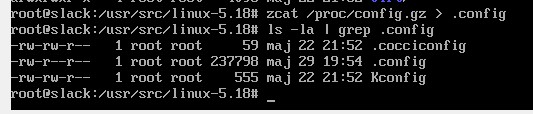
\includegraphics[width=8cm]{config copy.jpg}
\caption{Skopiowanie aktualnego configu}
\end{figure}

Po utworzeniu configu używamy komendy \textit{make localmodconfig} do stworzenia pliku konfiguracyjnego. Zostaniemy zapytani o to konfigurację poszczególnych modułów jądra, wszystko zostawiamy domyślnie. Wynik komendy:

\begin{figure}[H]
\centering
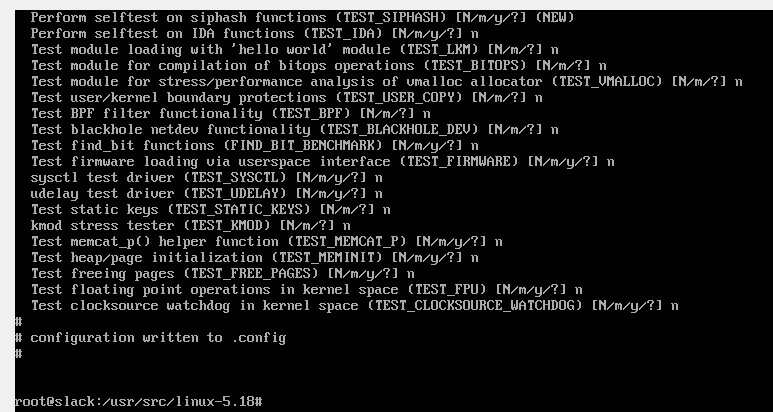
\includegraphics[width=8cm]{konfig jonder.jpg}
\caption{Zakończona konfiguracja jądra}
\end{figure}

Jesteśmy gotowi do kompilacji jądra. Użyta do tego została komenda \textit{make}::

\begin{figure}[H]
\centering
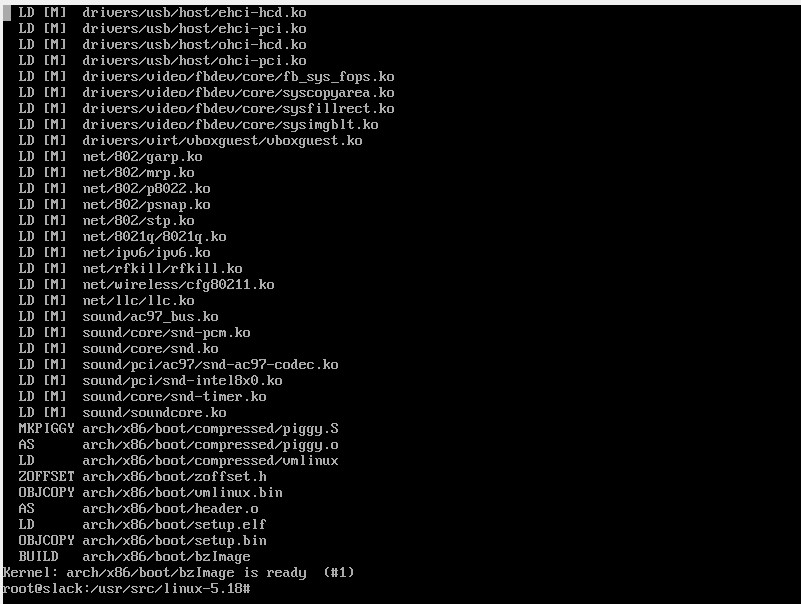
\includegraphics[width=8cm]{kompilacjajadra.jpg}
\caption{Zakończona kompilacja jądra}
\end{figure}

Po kompilacji jądra należy podobnie skompilować moduły komendą \texit{make modules}:

\begin{figure}[H]
\centering
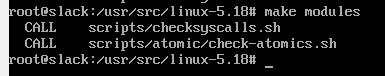
\includegraphics[width=8cm]{kompilacja-modulow.jpg}
\caption{Zakończona kompilacja modułów}
\end{figure}

Wykonujemy również komendę \textit{make modules_install} w celu wygenerowania komendy generującej ramdisk:

\begin{figure}[H]
\centering
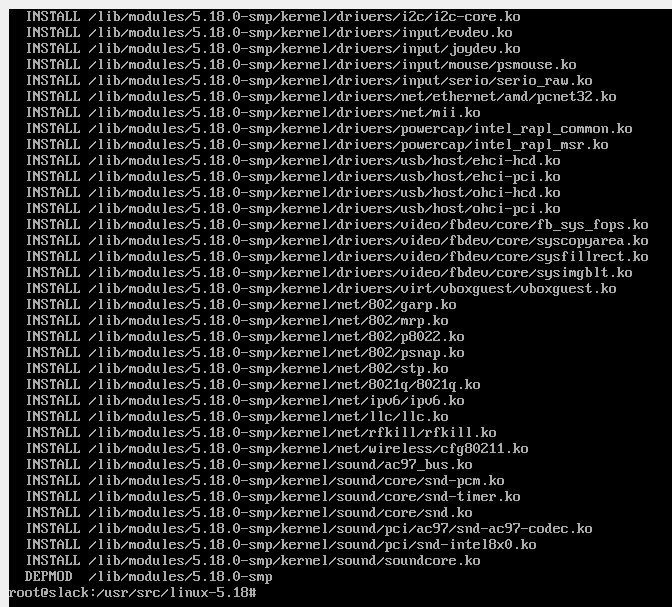
\includegraphics[width=8cm]{make install.jpg}
\caption{Komenda make install}
\end{figure}

Następnie należy skopiować pliki potrzebne do uruchomienia nowego jądra do katalogu /boot:

\begin{figure}[H]
\centering
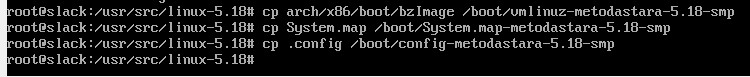
\includegraphics[width=8cm]{kopiowanieplikow.jpg}
\caption{Kopiowanie plików do katalogu boot}
\end{figure}

Po kopiowaniu jesteśmy gotowi do zlinkowania pliku System.map:

\begin{figure}[H]
\centering
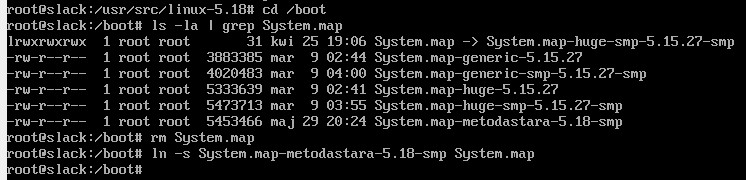
\includegraphics[width=8cm]{linksystemmap.jpg}
\caption{Podmienienie pliku System.map}
\end{figure}

Po linkowaniu możemy wygenerować komendę służącą do wygenerowania ramdisku:

\begin{figure}[H]
\centering
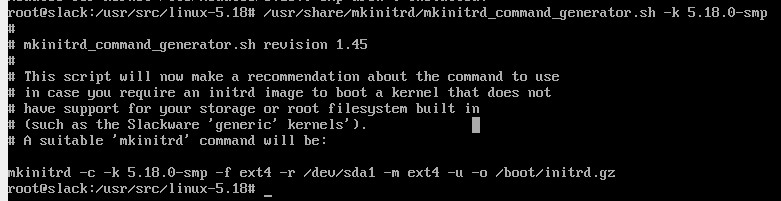
\includegraphics[width=8cm]{genramdisk.jpg}
\caption{Generowanie komendy do generacji ramdisk}
\end{figure}

Używamy teraz wygenerowanej komendy do utworzenia ramdisku:

\centering\textit{mkinitrd -c -k 5.18.0-smp -f ext4 -r /dev/sda1 -m ext4 -u -o /boot/initrd.gz}

\begin{figure}[H]
\centering
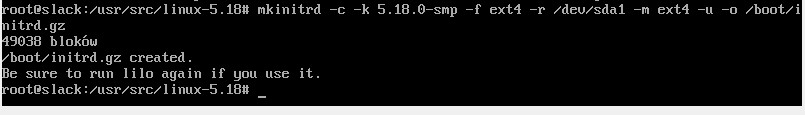
\includegraphics[width=8cm]{generateramdiskwtf.jpg}
\caption{Generowanie ramdisk}
\end{figure}

Aby ukazać wygenerowany plik lilo.conf używamy \textit{cat /etc/lilo.conf}:

\begin{figure}[H]
\centering
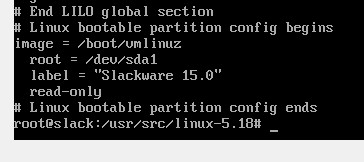
\includegraphics[width=8cm]{lilowtf.jpg}
\caption{Wygenerowany plik lilo.conf}
\end{figure}

Edytujemy plik w celu ustawienia nowego kernela i uruchamiamy komendę lilo:

\begin{figure}[H]
\centering
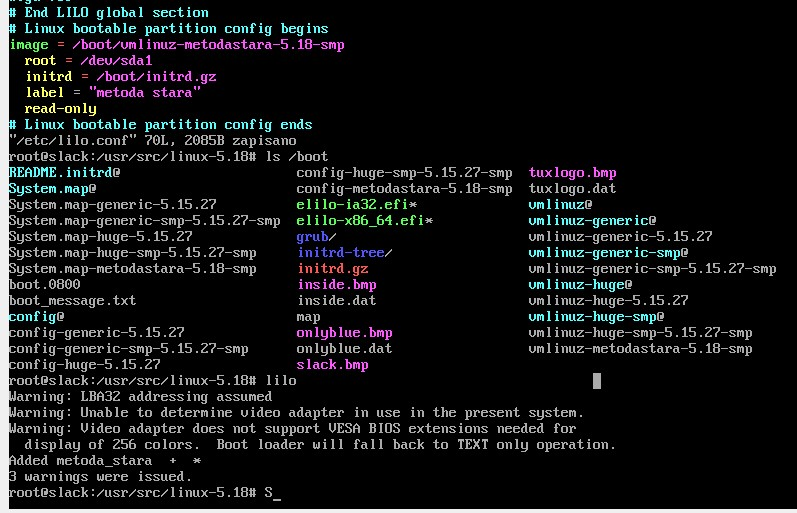
\includegraphics[width=8cm]{liloafter.jpg}
\caption{Edycja i uruchomienie lilo}
\end{figure}

Jesteśmy gotowi zrestartować maszynę. Wpis pojawił się przy uruchamianiu:

\begin{figure}[H]
\centering
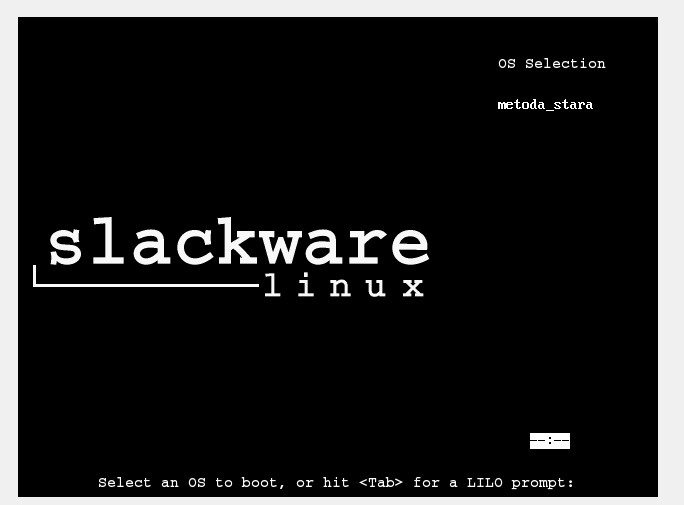
\includegraphics[width=8cm]{uruchamianielionuxa.jpg}
\caption{Uruchamianie nowego jądra}
\end{figure}

Po zalogowaniu widzimy, że nowe jądro zostało prawidłowo uruchomione:

\begin{figure}[H]
\centering
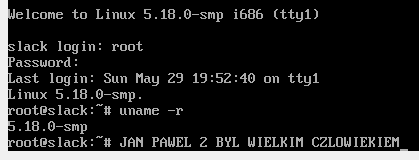
\includegraphics[width=8cm]{sprawdzeniedzialaniametodastara.png}
\caption{Sprawdzenie działania jądra}
\end{figure}

\section{Metoda nowa - streamline_config.pl}

Należy wygenerować plik konfiguracyjny zgodnie z instrukcją:

\begin{figure}[H]
\centering
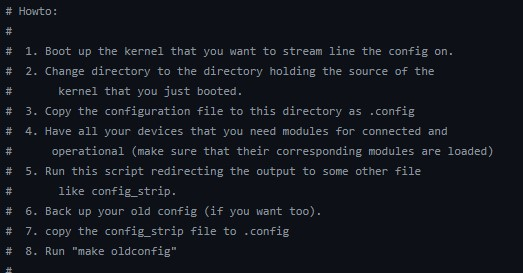
\includegraphics[width=8cm]{instrukcja.jpg}
\caption{Instrukcja wygenerowania skryptu}
\end{figure}

Wykonujemy kilka komend niezbędnych do przygotowania środowiska:

\begin{figure}[H]
\centering
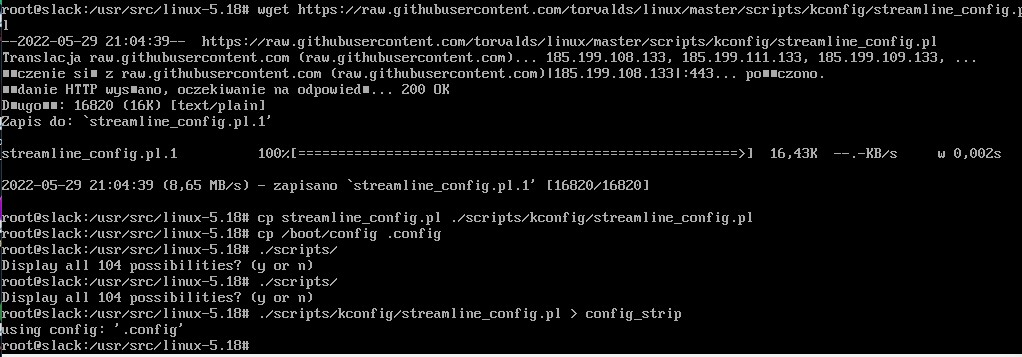
\includegraphics[width=8cm]{przygotowaniestreamline.jpg}
\caption{Przygotowanie środowiska}
\end{figure}

Po konfiguracji wykonujemy \textit{make oldconfig} jak każe instrukcja:

\begin{figure}[H]
\centering
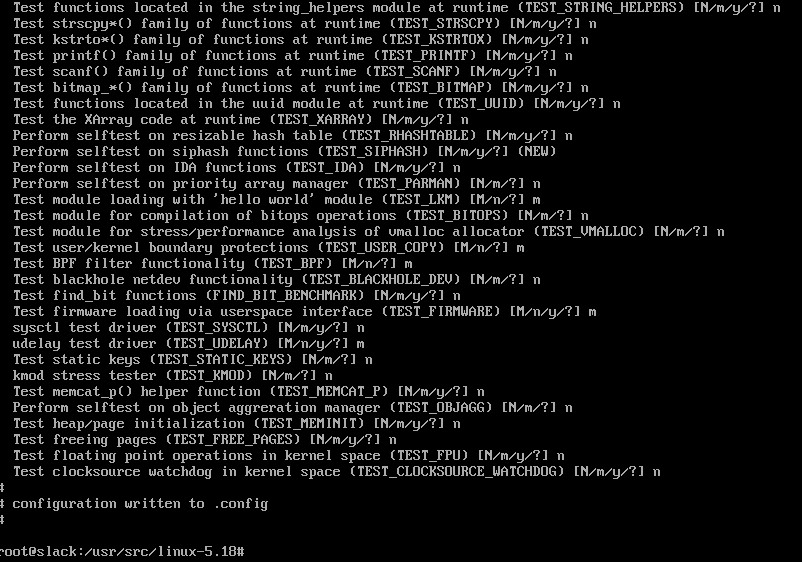
\includegraphics[width=8cm]{makeoldconfig.jpg}
\caption{Wykonanie komendy make oldconfig}
\end{figure}

Następnie ponownie wykonujemy kompilację jądra i modułów oraz ich instalację komendą \textit{make && make modules && make modules_install}

\begin{figure}[H]
\centering
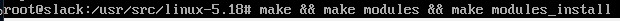
\includegraphics[width=8cm]{makemakemake.jpg}
\caption{Kompilacja i instalacja jądra i modułów}
\end{figure}

\begin{figure}[H]
\centering
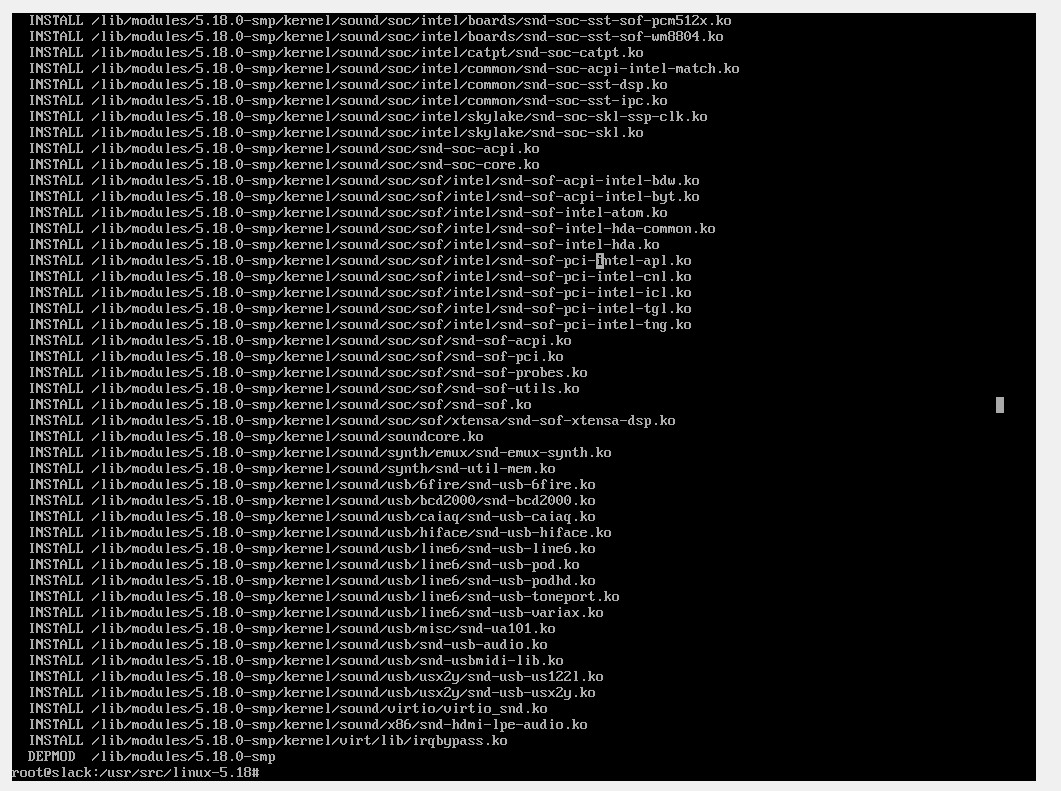
\includegraphics[width=8cm]{pokompilacji.jpg}
\caption{Wynik kompilacji i instalacji jądra/modułów}
\end{figure}

Wykonujemy następnie ten sam krop co w poprzedniej metodzie, to znaczy kopiujemy niezbędne pliki do katalogu /boot i tworzymy dowiązanie System.map:

\begin{figure}[H]
\centering
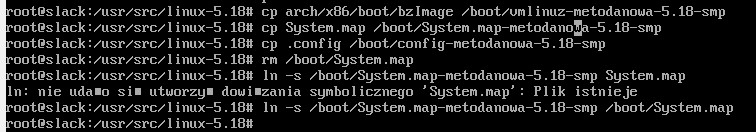
\includegraphics[width=8cm]{dowiazaniaxd.jpg}
\caption{Przekopiowanie plików konfiguracyjnych i stworzenie dowiązań}
\end{figure}

Analogicznie tworzymy też ramdisk:

\begin{figure}[H]
\centering
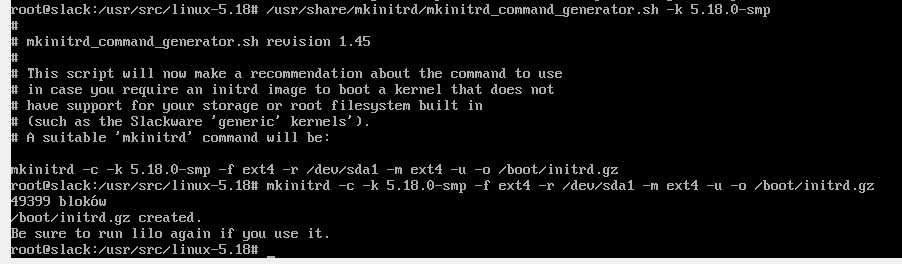
\includegraphics[width=8cm]{ramdiskkekw.jpg}
\caption{Stworzenie ramdisk}
\end{figure}

Dodajemy kolejny wpis oznaczający nową metodę do /etc/lilo.conf

\begin{figure}[H]
\centering
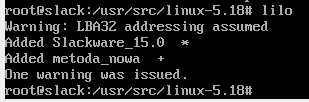
\includegraphics[width=8cm]{lilokomenda.jpg}
\caption{Nowe wejście w lilo.conf}
\end{figure}

Jesteśmy gotowi zrestartować maszynę i sprawdzić działanie nowego jądra. Nowy kernel pojawił się w menu wyboru:

\begin{figure}[H]
\centering
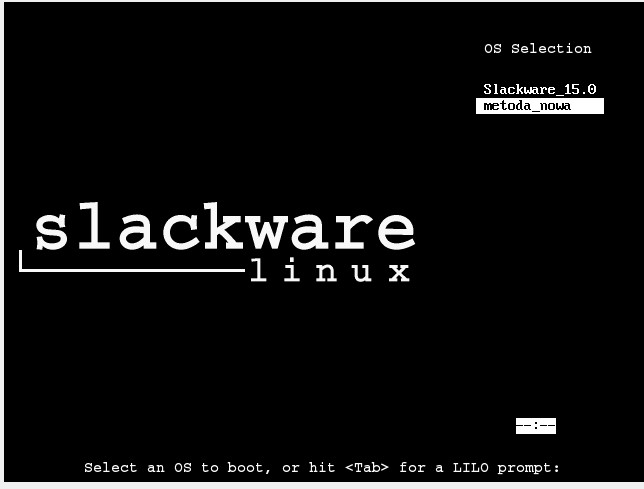
\includegraphics[width=8cm]{bootentry.jpg}
\caption{Nowe jądro w oknie wyboru}
\end{figure}

System uruchomił się i działa poprawnie. Sprawdzamy wersję kernela aby upewnić się, że uruchomiliśmy prawidłową wersją komendą \textit{uname -r}:

\begin{figure}[H]
\centering
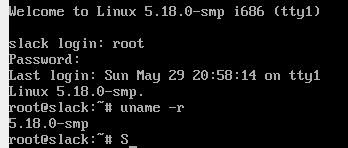
\includegraphics[width=8cm]{newkernelwtf.jpg}
\caption{Test nowego jądra}
\end{figure}

\section{Podsumowanie}

Kompilacja jądra obydwoma sposobami była podobna. Zdecydowanie bardziej jednak podobała mi się kompilacja drugim, nowszym sposobem. Była odrobinę prostsza, trwała jednak kilka razy dłużej mimo tych samych ustawień maszyny wirtualnej.

Jedynym napotkanym problemem był problem z podaniem wersji kernela przy generowaniu komendy do utworzenia ramdisku. Okazało się, że przy podawaniu wersji należało podać ją z 0 na końcu, tj. 5.18.0 zamiast samego 5.18. Był to problem stosunkowo łatwy do rozwiązania, wystarczyło spojrzeć na wynik kompilacji jądra.

\end{document}
